\documentclass[tikz,border=12pt]{standalone}
\usepackage{amsmath}
\usepackage{amssymb}
\usepackage{tikz}

\definecolor{ink}{HTML}{0F172A}
\definecolor{linegray}{HTML}{64748B}
\definecolor{visible}{HTML}{E2E8F0}
\definecolor{masked}{HTML}{F8FAFC}
\definecolor{maskedge}{HTML}{94A3B8}
\definecolor{prediction}{HTML}{F1F5F9}
\definecolor{lossfill}{HTML}{CBD5E1}

\begin{document}
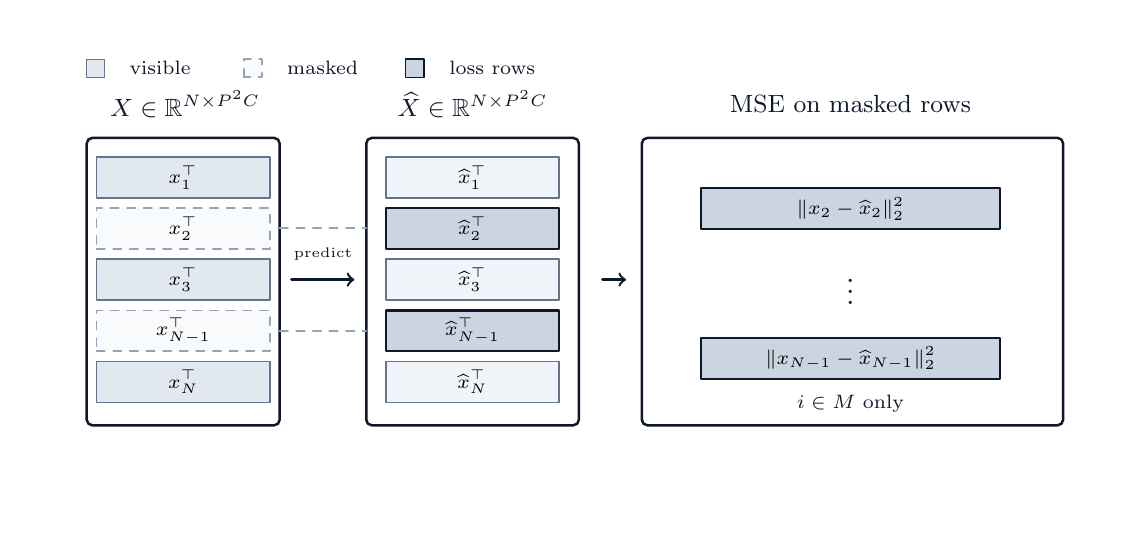
\begin{tikzpicture}[
  font=\sffamily,
  line cap=round,
  line join=round,
  row/.style={
    draw=linegray,
    line width=0.6pt,
    minimum width=2.2cm,
    minimum height=0.52cm,
    inner sep=2pt,
    align=center,
    font=\scriptsize
  },
  masked row/.style={
    row,
    draw=maskedge,
    dashed,
    fill=masked
  },
  prediction row/.style={
    row,
    fill=prediction
  },
  loss row/.style={
    row,
    draw=ink,
    line width=0.85pt,
    fill=lossfill
  },
  loss term/.style={
    loss row,
    minimum width=3.8cm
  }
]
  \fill[white] (-0.55,-0.65) rectangle (13.0,5.55);

  % Target patch matrix.
  \node[ink, font=\small] at (1.45,4.58)
    {$X \in \mathbb{R}^{N\times P^2 C}$};
    \draw[ink, line width=0.9pt, rounded corners=2pt]
      (0.2,0.5) rectangle (2.65,4.15);
    \node[row, fill=visible] at (1.425,3.65) {$x_1^\top$};
    \node[masked row] at (1.425,3.0) {$x_2^\top$};
    \node[row, fill=visible] at (1.425,2.35) {$x_3^\top$};
    \node[masked row] at (1.425,1.7) {$x_{N-1}^\top$};
    \node[row, fill=visible] at (1.425,1.05) {$x_N^\top$};

  % Reconstructed patch matrix.
    \node[ink, font=\small] at (5.1,4.58)
      {$\widehat{X} \in \mathbb{R}^{N\times P^2 C}$};
    \draw[ink, line width=0.9pt, rounded corners=2pt]
      (3.75,0.5) rectangle (6.45,4.15);
    \node[prediction row] at (5.1,3.65) {$\widehat{x}_1^\top$};
    \node[loss row] at (5.1,3.0) {$\widehat{x}_2^\top$};
    \node[prediction row] at (5.1,2.35) {$\widehat{x}_3^\top$};
    \node[loss row] at (5.1,1.7) {$\widehat{x}_{N-1}^\top$};
    \node[prediction row] at (5.1,1.05) {$\widehat{x}_N^\top$};

  % The loss is evaluated only on the masked rows.
    \draw[ink, ->, line width=0.9pt] (2.8,2.35) -- (3.6,2.35);
    \node[ink, font=\tiny, fill=white, inner sep=1.5pt]
      at (3.2,2.68) {predict};
    \draw[maskedge, dashed, line width=0.7pt]
      (2.65,3.0) -- (3.75,3.0);
    \draw[maskedge, dashed, line width=0.7pt]
      (2.65,1.7) -- (3.75,1.7);
    \draw[ink, ->, line width=0.9pt] (6.75,2.35) -- (7.05,2.35);

    \node[ink, font=\small] at (9.9,4.58) {MSE on masked rows};
  \draw[ink, line width=0.9pt, rounded corners=2pt]
    (7.25,0.5) rectangle (12.6,4.15);
    \node[loss term] at (9.9,3.25)
       {$\lVert x_2-\widehat{x}_2\rVert_2^2$};
  \node[ink, font=\large] at (9.9,2.3) {$\vdots$};
  \node[loss term] at (9.9,1.35)
    {$\lVert x_{N-1}-\widehat{x}_{N-1}\rVert_2^2$};
  \node[ink, font=\scriptsize] at (9.9,0.78)
    {$i\in M\ \text{only}$};

  % Legend shared with the masking figures.
  \fill[visible] (0.2,4.92) rectangle (0.43,5.15);
  \draw[linegray, line width=0.45pt] (0.2,4.92) rectangle (0.43,5.15);
  \node[ink, font=\scriptsize, anchor=west] at (0.62,5.04) {visible};
  \fill[masked] (2.2,4.92) rectangle (2.43,5.15);
  \draw[maskedge, dashed, line width=0.7pt]
    (2.2,4.92) rectangle (2.43,5.15);
  \node[ink, font=\scriptsize, anchor=west] at (2.62,5.04) {masked};
  \fill[lossfill] (4.25,4.92) rectangle (4.48,5.15);
  \draw[ink, line width=0.55pt] (4.25,4.92) rectangle (4.48,5.15);
  \node[ink, font=\scriptsize, anchor=west] at (4.68,5.04) {loss rows};
\end{tikzpicture}
\end{document}
